

\begin{frame}{Uso de GridLayout en Android}
\textbf{¿Qué es GridLayout?}

\begin{itemize}
    \item Es un contenedor de diseño (ViewGroup) que organiza los elementos en una cuadrícula de filas y columnas.
    \item Permite ubicar componentes de manera estructurada y alineada.
\end{itemize}

\vspace{0.4cm}

\textbf{¿Para qué sirve?}
\begin{itemize}
    \item Diseñar interfaces organizadas en forma de tabla.
    \item Alinear múltiples elementos (botones, imágenes, textos) fácilmente.
    \item Crear interfaces dinámicas como teclados, galerías o tableros de juego.
\end{itemize}

\vspace{0.4cm}

\textbf{Características principales:}
\begin{itemize}
    \item Define número de filas y columnas.
    \item Permite que los elementos ocupen múltiples celdas (rowSpan, columnSpan).
    \item Soporta alineación y distribución del espacio.
\end{itemize}


\end{frame}


\begin{frame}[fragile]
\frametitle{Demo 03: Agregar un Panel de Botones utilizando un GridLayout}
\begin{columns}
\column{0.80\linewidth}
Del Repositorio Github:
\begin{itemize}
\item Copiar el archivo MainActivity\_Demo03.java (dentro del Folder códigosJAVA) al mismo directorio donde esta el MainActivity.java
\item Copiar el archivo activity\_main\_demo03.xml (dentro del Folder Carpeta\_layout) al mismo directorio donde esta el activity\_main.xml
\item Modificar en el archivo AndroidManifest.xml la cadena \textit{.MainActivity\_Demo02} por \textit{.MainActivity\_Demo03}
\end{itemize}

\begin{block}{Demo \#03}
Muestra una App con un panel de botones, que muestra un Toast para cada boton presionado por el usuario.  
\end{block}


\column{0.20\linewidth}

\begin{center}
 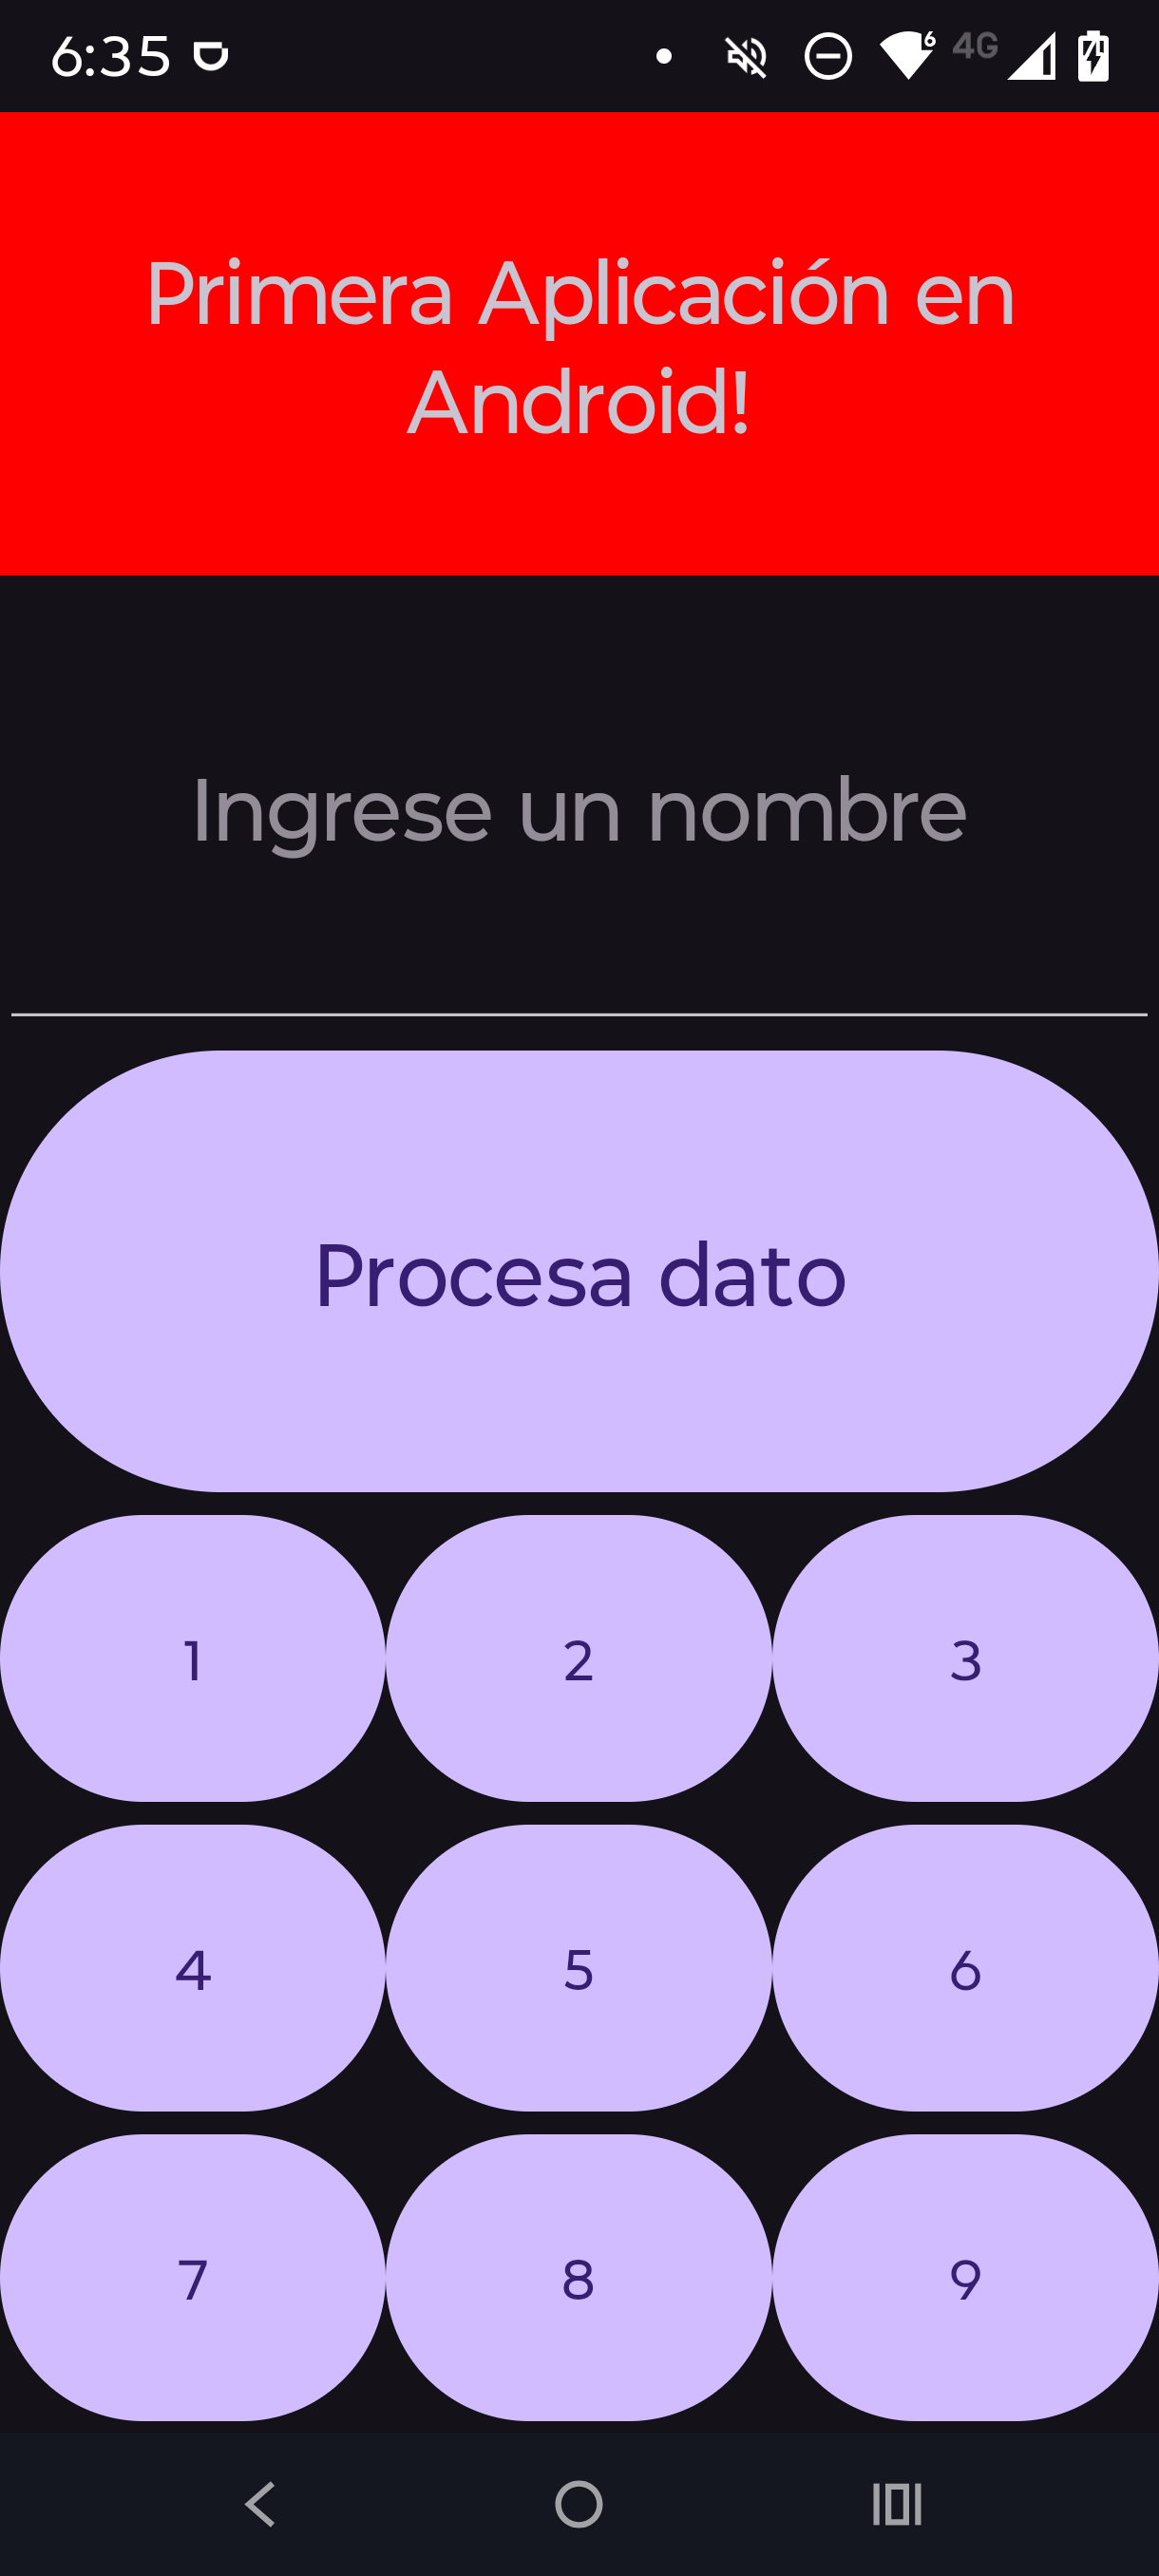
\includegraphics[width=0.98\textwidth]{02_TallerCBTis/figs/Demo03}
\end{center}

\end{columns}

\end{frame}


